\documentclass[]{article}   % list options between brackets

\usepackage{color}
\usepackage{graphicx}
%% The amssymb package provides various useful mathematical symbols
\usepackage{amssymb}
%% The amsthm package provides extended theorem environments
\usepackage{amsthm}
\usepackage{amsmath}
\usepackage{hyperref}

\newtheorem{axiom}{Axiom}

\newtheorem{proposition}{Proposition}
\newtheorem{definition}{Definition}

\def\shownotes{1}
\def\notesinmargins{0}

\ifnum\shownotes=1
\ifnum\notesinmargins=1
\newcommand{\authnote}[2]{\marginpar{\parbox{\marginparwidth}{\tiny %
  \textsf{#1 {\textcolor{blue}{notes: #2}}}}}%
  \textcolor{blue}{\textbf{\dag}}}
\else
\newcommand{\authnote}[2]{
  \textsf{#1 \textcolor{blue}{: #2}}}
\fi
\else
\newcommand{\authnote}[2]{}
\fi

\newcommand{\knote}[1]{{\authnote{\textcolor{green}{Alex notes}}{#1}}}
\newcommand{\dnote}[1]{{\authnote{\textcolor{red}{Dima notes}}{#1}}}
\newcommand{\vnote}[1]{{\authnote{\textcolor{purple}{Vasily notes}}{#1}}}

\newcommand{\term}[1]{\textit{#1}}

% type user-defined commands here
\usepackage[T1]{fontenc}

\usepackage{xcolor}
\usepackage{graphicx}
\usepackage[margin=1in]{geometry}
\usepackage{titlesec}

\definecolor{dkgreen}{rgb}{0,0.6,0}
\definecolor{gray}{rgb}{0.5,0.5,0.5}
\definecolor{mauve}{rgb}{0.58,0,0.82}


\newtheorem{claim1}{Claim}
\newtheorem{dfn}{Definition}
\newtheorem{defn}{Definition}
\newcommand{\ma}{\mathcal{A}}
\newcommand{\mb}{\mathcal{B}}
\newcommand{\he}{\hat{e}}
\newcommand{\sr}{\stackrel}
\newcommand{\ra}{\rightarrow}
\newcommand{\la}{\leftarrow}

\newcommand{\ignore}[1]{} % may contain useful stuff (that needs more work)
\newcommand{\full}[1]{} % use only for full version
\newcommand{\notfull}[1]{#1}
\newcommand{\rand}{\stackrel{R}{\leftarrow}}
\newcommand{\haya}{blue}
\newcommand{\amitabh}{purple}
\newcommand{\questions}{blue}
\newcommand{\defined}{\stackrel{\mbox{\tiny{def}}}{=}}
\newcommand{\mc}{\mathcal}
\newcommand{\ms}{\mathsf}
\newcommand{\txs}{\textsf}
\newcommand{\lea}{\leftarrow}
\newcommand{\rea}{\rightarrow}
\newcommand{\adv}{{\cal A} }
\def\kg{{\sf{Gen}}}
\def\enc{{\sf{Enc}}}
\def\dec{{\sf{Dec}}}
\newcommand{\btc}{\includegraphics[height=8pt]{assets/btc.jpg}}
\newcommand{\mypar}[1]{\smallskip\noindent\textbf{#1.}\ \ \ }

\newcommand{\dlog}{dlog(h)}
\newcommand{\pedersen}{pcom(h, c)}
\newcommand{\height}{\mathcal{H}}
\newcommand{\ergo}{Ergo}

\newcommand{\ecash}{$\Sigma$-Cash}

\newcommand{\edata}{$\Sigma$-Data}

\newcommand{\state}{\textit{State}}
\newcommand{\roller}{\textbf{Rollerchain}}
\newcommand{\popow}{\textbf{PoPoW}}
\newcommand{\ads}{\textbf{ADS}}

% as we do not know which term to use for a state element, we use a command for this
\newcommand{\coin}{box}
\newcommand{\Coin}{Box}

\newcommand{\sigm}{sigma}

\newcommand{\extract}[1]{$extract({#1})$}

\usepackage[utf8]{inputenc}

\usepackage{minted}
\usemintedstyle{manni}
\usepackage{microtype}


\begin{document}

\title{The \ergo{} Yellow Paper}
\author{Ergo Developers}
%\author{Alexander Chepurnoy \and Nazeem Faour \and Dmitry Meshkov}
\maketitle

\newpage
\tableofcontents


\part{Introduction}
\label{part-intro}

This document describes a blockchain protocol named Ergo Platform~(or just Ergo) and a corresponding
reference implementation. Ergo is a conservative Proof-of-Work blockchain with ultimate new contract language~(called
ErgoTree, but in most cases you need a higher-level language, for example, ErgoScript) and better support for lightweight
and secure modes of operation.

\section{Vision}

\knote{Write what is Ergo in general, why is it needed and for whom.}


\subsection{State-Oriented Design}
\knote{Write about boxes as first-class citizens.}



\part{The Protocol}
\label{part-protocol}


\section{Notation and Preliminaries}

\subsection{A Note on Notation}

\knote{say about coin/box/output}


\section{Cryptographic Primitives}

We use Blake2b hash function with 256 bits output.

\knote{describe a curve used}


\section{Modes of Operation}
Ergo (since the very first testing network Testnet0) is supporting multiple security models. In addition to full node
mode, which is similar to Bitcoin fullnode, Ergo reference implementation supports Light-SPV, Light-Fullnode and Pruned-Fullnode modes.

\subsection{Full-Node Mode}
Like in Bitcoin, a full node is storing all the full blocks since genesis block. Full node checks proofs of work, linking structure correctness (parent block id, interlink elements), and all the transactions in all the blocks. A fullnode is storing all the full blocks forever. It is also holding full UTXO set to be able to validate an arbitrary transaction.
The only optimization a fullnode is doing is that is skipping downloading and checking AD-transformation block part (see below in the "Light-Fullnode" section).
For the full node regime, modifiers processing workflow is as follows:
\begin{enumerate}
   \item Send ErgoSyncInfo message to connected peers.
   \item Get response with INV message, containing ids of blocks, better than our best block.
   \item Request headers for all ids from 2.
   \item On receiving header:
   \begin{minted}{java}
if(history.apply(header).isSuccess) {
    if(!isInitialBootstrapping) Broadcast INV for this header
    Request transaction ids from this block
 } else {
    blacklist peer
 }
\end{minted}
\vspace{1em}

 % Mempool.apply(transactionIdsForHeader)
   \item On receiving transaction ids from header:
   \begin{minted}{java}
  transactionIdsForHeader.filter(txId => !MemPool.contains(txId)).foreach { txId =>
    request transaction with txId
  }
   \end{minted}
   \item On receiving a transaction:
   \begin{minted}{java}
   if(Mempool.apply(transaction).isSuccess) {
    if(!isInitialBootstrapping) Broadcast INV for this transaction
    Mempool.getHeadersWithAllTransactions { BlockTransactions =>
       GOTO 7
    }
 }
   \end{minted}
   \item Now we have BlockTransactions: all transactions corresponding to some Header
   \begin{minted}{java}
    if(History.apply(BlockTransactions) == Success(ProgressInfo)) {
      if(!isInitialBootstrapping) Broadcast INV for BlockTransactions
     /*We should notify our neighbours, that now we have all the transactions
     State apply modifiers (may be empty for block in a fork chain)
     and generate ADProofs for them.
     TODO requires different interface from scorex-core,
     because it should return ADProofs
     TODO when minimal state apply Progress info,
     it may also create UTXOSnapshot
     (e.g. every 30000 blocks like in Ethereum).
     This UTXOSnapshot should be required for mining by Rollerchain*/
     if(State().apply(ProgressInfo) == Success((newState, ADProofs))) {
       if("mode"="full" || "mode"=="pruned-full") ADProofs.foreach ( ADProof => History.apply(ADProof))
       if("mode"=="pruned-full" || "mode"=="light-full") drop BlockTransactions and ADProofs older than BlocksToKeep
     } else {
       //Drop Header from history, because it's transaction sequence is not valid
       History.drop(BlockTransactions.headerId)
     }
  } else {
    blacklist peer who sent header
  }
   \end{minted}
\end{enumerate}

\subsection{Pruned Full-Node Mode}
This mode is similar to fast-sync in Geth or Grothendieck, warp-mode in Parity (all the three are Ethereum protocol clients), but makes more aggressive optimizations. In particular, a pruned-fullnode is not down- loading and storing full blocks not residing in a target blockchain suffix, and also removing full blocks going out of the suffix.
In detail, a pruned client is downloading all the headers, then, by using them, it checks proofs-of-work and linking structure(or parent id only?). Then it downloads a UTXO snapshot for some height from its peers. Finally, full blocks after the snapshot are to be downloaded and applied to get a current UTXO set.
A pruned fullnode is also skipping AD-transformation block part, like a fullnode. Additional setting: "suffix" - how much full blocks to store(w. some minimum set?).
Its regular modifiers processing is the same as for fullnode regime, while its bootstrap process is different:
\begin{enumerate}
\item Send ErgoSyncInfo message to connected peers.
\item Get response with INV message, containing ids of blocks, better than our best block.
\item Request headers for all ids from 2.
\item On receiving header:
\begin{minted}{java}
if(History.apply(header).isSuccess) {
    if(!(localScore == networkScore)) GOTO 1
    else GOTO 5
 } else {
    blacklist peer
 }
\end{minted}

\item Request historical UTXOManifest for at least BlocksToKeep back.

\item On receiving UTXOSnapshotManifest:

\begin{minted}{java}
UTXOSnapshotManifest.chunks.foreach { chunk =>
    request chunk from sender() //Or from random fullnode
  }
\end{minted}
\item On receiving UTXOSnapshotChunk:
\begin{minted}{java}
State.applyChunk(UTXOSnapshotChunk) match {
     case Success(Some(newMinimalState)) => GOTO 8
     case Success(None) => stay at 7
     /*we need more chunks to construct state.
     TODO periodicaly request missed chunks*/
     case Failure(e) => ???
     //UTXOSnapshotChunk or constcucted state roothash is invalid
  }
\end{minted}

\item Request BlockTransactions starting from State we have
\begin{minted}{java}
History.headersStartingFromId(State.headerId).foreach { header =>
    send message(GetBlockTransactionsForHeader(header)) to Random fullnode
  }
\end{minted}
\item On receiving BlockTransactions: same as in Fullnode.7 .
\item Operate as Fullnode.


\end{enumerate}

\subsection{Light Full-Node Mode}
This mode is based on an idea to use a 2-party authenticated dynamic dictionary built on top of UTXO set. A light-fullnode holds only a root digest of a dictionary. It checks all the full blocks, or some suffix of the full blockchain, depending on setting, thus starting from a trusted pre-genesis digest or some digest in the blockchain. A light-fullnode is using AD-transformations (authenticated dictionary transformations) block section containing batch-proof for UTXO transformations to get a new digest from an old one. It also checks all the transactions, but doesn’t store anything but a single digest for that. Details can be found in the paper https://eprint.iacr.org/2016/994. \par
Additional settings : "depth" - from which block in the past to check transactions (if 0, then go from genesis). \par
"additional-checks" - light-fullnode trusts previous digest and checks current digest validity by using the previous one as well as AD-transformations. \par
"additional-depth" - depth to start additional checks from.
\begin{enumerate}
\item Send ErgoSyncInfo message to connected peers.
\item Get response with INV message, containing ids of blocks, better than our best block.
\item Request headers for all ids from 2.
\item On receiving header:
\begin{minted}{java}
if(History.apply(header).isSuccess) {
    if(!(localScore == networkScore)) GOTO 1
    else GOTO 5
 } else {
    blacklist peer
 }
\end{minted}
\item Request BlockTransactions and ADProofs starting from BlocksToKeep back in History (just 1 last header after node botstrapping):
\begin{minted}{java}
History.lastBestHeaders(BlocksToKeep).foreach { header =>
    send message(GetBlockTransactionsForHeader(header)) to Random fullnode
    send message(GetAdProofsHeader(header)) to Random fullnode
  }
\end{minted}
\item On receiving modifier BlockTransactions or ADProofs:
\begin{minted}{java}
if(History.apply(modifier) == Success(ProgressInfo)) {
  /* TODO if history now contains both ADProofs and BlockTransactions,
  it should return ProgressInfo with both of them, otherwise
  it should return empty ProgressInfo */
if(State().apply(ProgressInfo) == Success((newState, ADProofs)))
{
if("mode"=="pruned-full") drop BlockTransactions and ADProofs older than BlocksToKeep
}
else {
         /*Drop Header from history, because it's transaction sequence is not valid*/
         History.drop(BlockTransactions.headerId)
     }
  }
\end{minted}
\end{enumerate}

\subsection{Light-SPV Mode}
This mode is not about checking any full blocks. Like in Bitcoin, an SPV node is downloading block headers only, and so checks only proofs of work and links. Unlike Bitcoin’s SPV, the Light-SPV is downloading and checking not all the headers but a sublinear(in blockchain length) number of them(in benchmarks, this is about just tens of kilobytes instead of tens or hundreds of megabytes for Bitcoin/Ethereum).
Light-SPV mode is intended to be useful for mobile phones and low-end hardware.
\subsubsection{Bootstrap}
\begin{enumerate}
\item Send GetPoPoWProof for all connections.
\item On receive PoPoWProof apply it to History (History should be able to determine, whether this PoPoWProof is better than it's current best header chain).
\item GOTO regular regime.
\end{enumerate}
\subsubsection{Regular}
\begin{enumerate}
\item Send ErgoSyncInfo message to connected peers
\item Get response with INV message, containing ids of blocks, better than our best block.
\item Request headers for all ids from 2.
\item On receiving header:
\begin{minted}{java}
 if(History.apply(header).isSuccess) {
    State.apply(header) // just change state roothash
    if(!isInitialBootstrapping) Broadcast INV for this header
 } else {
    blacklist peer
 }
\end{minted}
\end{enumerate}
\subsection{Mode-Related Settings}
Ergo has the following settings determines a mode:
\begin{itemize}
\item ADState: Boolean - keeps state roothash only.
\item VerifyTransactions: Boolean - download block transactions and verify them (requires BlocksToKeep == 0 if disabled).
\item PoPoWBootstrap: Boolean - download PoPoW proof only
\item BlocksToKeep: Int - number of last blocks to keep with transactions, for all other blocks it keep header
only. Keep all blocks from genesis if negative
\item MinimalSuffix: Int - minimal suffix size for PoPoW proof (may be pre-defined constant).
\end{itemize}
\par
‘if(VerifyTransactions == false) require(BlocksToKeep == 0)‘ Mode from "multimode.md" can be determined as follows:

\section{Ergo Block Structure}
Ergo block consists of 4 parts:

\begin{itemize}
    \item{\em Header } - minimal amount of data required to synchronize the chain and check PoW correctness.
    Also contains hashes of other sections.
    \item{\em BlockTransactions } - sequence of transactions, included in this block.
    \item{\em ADProofs } - proofs for transactions included into the corresponding BlockTransactions section of a block.
    Allows light clients to verify all the transactions and calculate new root hash.
    \item{\em Extension } - additional data, that does not correspond to previous sections.
    May contain interlinks, current miner votes and (sometimes) current parameters of the chain.
\end{itemize}

\subsection{Header}
\vspace{1em}
\begin{tabular}{ |p{2.5cm}||p{0.5cm}|p{7.5cm}|  }
    \hline
    \hline
    Field & Size & Description  \\
    \hline
    version  &  1 &  block version, to be increased on every soft- and hardfork  \\
    \hline
    parentId &  32 &  id of parent block  \\
    \hline
    ADProofsRoot &  32 &  hash of ADProofs for transactions in a block \\
    \hline
    stateRoot &  32 &  root hash (for an AVL+ tree) of a state after block application  \\
    \hline
    transactionsRoot  &  32 &  root hash (for a Merkle tree) of transactions in a block  \\
    \hline
    timestamp &  8 &  block timestamp(in milliseconds since beginning of Unix Epoch)  \\
    \hline
    nBits &  8 & current difficulty in a compressed view  \\
    \hline
    height &  4 & block height  \\
    \hline
    extensionRoot & 32 & root hash of extension section  \\
    \hline
    powSolution & 75-107 (depends on d) & solution of Autolykos PoW puzzle  \\
    \hline
\end{tabular}

\vspace{1em}
Some of these fields may be calculated by node by itself if it is in a certain mode:

\begin{itemize}
    \item parentId: if(status==bootstrap AND PoPoWBootstrap == false).
    \item interlinksRoot: if(PoPoWBootstrap == false).
    \item ADProofsRoot: if(status==regular AND ADState==false AND BlocksToKeep>0).
    \item stateRoot: if(status==regular AND ADState==false AND BlocksToKeep>0).
\end{itemize}

\subsection{Extension}

Extension is a key-value storage for a variety of data.
It contains 2 parts:
\begin{itemize}
    \item{\em Mandatory fields } - fields which keys are set via consensus rules and may be changed
    via soft/hard forks only. These fields have 4 bytes key and at most 64 bytes value.
    Value length is known for all peers and this limit only important due to soft forks -
    it is allowed to add at most 1 new key to this section per epoch (256 blocks between
    difficulty recalculation), if key is not known to a peer it assumes that soft fork that
    added this key was performed.
    \item{\em Optional fields } - random data miner may add to a block. This section contains at most 2
    elements with 32 byte key size and at most 64 byte value size.
\end{itemize}



\section{Ergo Modifiers Processing}


This section describes processing algorithm for Ergo modifiers in all security modes. Unlike most of blockchain systems, Ergo have the following types of modifiers: In-memory:
\begin{enumerate}
\item In-memory:
\begin{itemize}
\item Transaction - in-memory modifier.
\item TransactionIdsForHeader - ids of transactions in concrete block.
\item UTXOSnapshotManifest - ids of UTXO chunks and
\end{itemize}
\item Persistent:
\begin{itemize}
\item BlockTransactions - Sequence of transactions, corresponding to 1 block.
\item ADProofs - proof of transaction correctness relative to corresponding UTXO.
\item Header, that contains data required to verify PoW, link to previous block, state root hash and root hash to it's payload (BlockTransactions, ADProofs, Interlinks ...).
\item UTXOSnapshotChunk - part of UTXO.
\item PoPoWProof
\end{itemize}
Ergo will have the following parameters, that will determine concrete security regime:
\begin{itemize}
\item ADState: Boolean - keep state roothash only.
\item VerifyTransactions: Boolean - download block transactions and verify them (requires BlocksToKeep == 0 if disabled).
\item PoPoWBootstrap: Boolean - download PoPoW proof only.
\item BlocksToKeep: Int - number of last blocks to keep with transactions, for all other blocks it keep header only. Keep all blocks from genesis if negative.
\item MinimalSuffix: Int - minimal suffix size for PoPoW proof (may be pre-defined constant).
\begin{minted}{java}
if(VerifyTransactions == false) require(BlocksToKeep == 0)
\end{minted}
\end{itemize}
Mode from "multimode.md" can be determined as follows:
\begin{minted}{java}
mode = if(ADState == false && VerifyTransactions == true
&& PoPoWBootstrap == false && BlocksToKeep < 0) "full"
else if(ADState == false && VerifyTransactions == true
&& PoPoWBootstrap == false && BlocksToKeep >= 0) "pruned-full"
else if(ADState == true && VerifyTransactions == true
&& PoPoWBootstrap == false) "light-full"
else if(ADState == true && VerifyTransactions == false
&& PoPoWBootstrap == true && BlocksToKeep == 0) "light-spv"
else if(ADState == true && VerifyTransactions == true
&& PoPoWBootstrap == true && BlocksToKeep == 0) "light-full-PoPoW"
else //Other combinations are possible
\end{minted}
\end{enumerate}
\subsection{Modifiers processing}
\begin{minted}{java}
def updateHeadersChainToBestInNetwork() = {
  1.2.1. Send ErgoSyncInfo message to connected peers
  1.2.2. Get response with INV message,
  containing ids of blocks, better than our best block
  1.2.3. Request headers for all ids from 1.2.2.
  1.2.4. On receiving header
   if(History.apply(header).isSuccess) {
      if(!(localScore == networkScore)) GOTO 1.2.1
   } else {
      blacklist peer
      GOTO 1.2.1
   }
}
\end{minted}

\subsection{bootstrap}
\subsubsection{Download headers:}
\begin{minted}{java}
if(PoPoW) {
 1.1.1. Send GetPoPoWProof(suffix = Max(MinimalSuffix ,BlocksToKeep)) for all connections
 1.1.2. On receive PoPoWProof apply it to History
  /*
  History should be able to determine,
  whether this PoPoWProof is better, than it's current best header chain */
} else {
  updateHeadersChainToBestInNetwork()
}
\end{minted}
\subsubsection{Download initial State to start process transactions:}
\begin{minted}{java}
if(ADState == true) {
  Initialize state with state roothash from block header BlocksToKeep ago
} else if(BlocksToKeep < 0 || BlocksToKeep > History.headersHeight) {
  Initialize state with genesis State
} else {
/*
We need to download full state BlocksToKeep back in history
TODO what if we can download state only "BlocksToKeep - N"
or "BlocksToKeep + N" blocks back?
*/
  2.1. Request historical UTXOSnapshotManifest for at least BlocksToKeep back
  2.2. On receiving UTXOSnapshotManifest:
    UTXOSnapshotManifest.chunks.foreach ( chunk => request chunk from sender()
/*Or from random fullnode*/
  2.3. On receiving UTXOSnapshotChunk
  State.applyChunk(UTXOSnapshotChunk) match {
     case Success(Some(newMinimalState)) => GOTO 3
     case Success(None) => stay at 2.3
     /*we need more chunks to construct state. TODO periodicaly request missed chunks*/
     case Failure(e) => ???
     /*UTXOSnapshotChunk or constcucted state roothash is invalid*/
  }
}
\end{minted}
\subsubsection{Update State to best headers height:}
\begin{minted}{java}
 if(State.bestHeader == History.bestHeader) {
    //Do nothing, State is already updated
  } else if(VerifyTransactions == false) {
/*Just update State rootshash to best header in history*/
    State.setBestHeader(History.bestHeader)
  } else {
/*we have headers chain better than full block */
    3.1.
      assert(history contains header chain from State.bestHeader to History.bestHeaders)
      History.continuation(from = State.bestHeader, size = ???).get.foreach { header =>
        sendToRandomFullNode(GetBlockTransactionsForHeader(header))
        if(ADState == true) sendToRandomFullNode(GetADProofsForHeader(header))
      }
    3.2. On receiving modifiers ADProofs or BlockTransactions
      /*TODO History should return non-empty ProgressInfo
      only if it contains both ADProofs and BlockTransactions,
      or it contains BlockTransactions and ADState==false*/
      if(History.apply(modifier) == Success(ProgressInfo)) {
        if(State().apply(ProgressInfo) == Success((newState, ADProofs))) {
          if(ADState==false) ADProofs.foreach ( ADProof => History.apply(ADProof))
          if(BlocksToKeep>=0)
          /*remove BlockTransactions and ADProofs older than BlocksToKeep from history*/
        } else {
      /*Drop Header from history,
      because it's transaction sequence is not valid*/
          History.drop(modifier.headerId)
        }
      } else {
        blacklistPeer
      }
      GOTO 3
    }
\end{minted}
\subsubsection{GOTO regular mode.}
\begin{minted}{java}

\end{minted}
\subsection{Regular}
Two infinite loops in different threads with the following functions inside:
\begin{enumerate}
\item UpdateHeadersChainToBestInNetwork()
\item Download and update full blocks when needed
\end{enumerate}
\begin{minted}{java}
 if(State.bestHeader == History.bestHeader) {
    //Do nothing, State is already updated
  } else if(VerifyTransactions == false) {
    //Just update State rootshash to best header in history
    State.setBestHeader(History.bestHeader)
  } else {
    //we have headers chain better then full block
    3.1. Request transaction ids from all headers without transactions
      assert(history contains header chain from State.bestHeader to History.bestHeaders)
      History.continuation(from = State.bestHeader, size = ???).get.foreach { header =>
        sendToRandomFullNode(GetTransactionIdsForHeader(header))
        if(ADState == true) sendToRandomFullNode(GetADProofsForHeader(header))
      }
    3.2. On receiving TransactionIdsForHeader:
      Mempool.apply(TransactionIdsForHeader)
      TransactionIdsForHeader.filter(txId => !MemPool.contains(txId)).foreach { txId =>
        request transaction with txId
      }
    3.3. On receiving a transaction:
      if(Mempool.apply(transaction).isSuccess) {
         Broadcast INV for this transaction
         Mempool.getHeadersWithAllTransactions { BlockTransactions =>
            GOTO 3.4 //now we have BlockTransactions
         }
      }
    3.4. (same as 3.2. from bootstrap)
  }
\end{minted}


\section{Economic survivability}

We outline 2 properties required for a long-term survivability of the chain:

\begin{itemize}
    \item{} Coins which no one can spent (e.g. because keys are lost)
    should be returned into circullation. Otherwise, after the end of the initial coins emission, amount of the coins
    in the circullation always decreases and will eventually reach 0.
    \item{} Nothing should be kept in the state forever and for free.
    Otherwise, the size of the state is always increasing in the the long, reducing clients performance
    and thus increasing requirements to run a client.
\end{itemize}

To achieve this, we propose the following modifications to the consensus rules.
Register $R2$ of the box will contain tuple $(tx\_id, out\_num,
last\_height)$. $last\_height$ field is used to determine the block height
at the moment of transaction generation. Transaction can only be put in the
block of height $h$ if for every created box $h - max\_drift < R2.last\_height < h$.

Once the subsidized period for the box ends (that is,
$current\_block\_height \ge R2.last\_height + SP$), anyone can
create the new box with the exactly the same content (including the guarding
script) except the monetary value and $R2$ content. The monetary value is
reduced by no more $K \cdot B$, where $B$ is the box size and $K$ is the storage cost of one byte.
Thus, at most $K \cdot B$ coins are to be paid to a miner.
If box value is less that $K \cdot B$, all box content including tokens goes to miner.

%$last\_height$ is replaced with the new height that is at least
%$current\_block\_height - max\_drift$, so that the subsidized period starts over.

We propose the following concrete parameters:
\begin{itemize}
    \item{} $K$ - cost of storage of 1 byte of data in a State for 1 block.
    Should be determined by miner votes, $10^{-6} (Ergo/byte)$ by default.
    \item{} $max\_drift$ - maximum amount of time difference between transaction
    creation and its inclusion into the blockchain.
    It is predefined constant $max\_drift = 2016 = 3$ days.
    \item{} $SP$ - number of blocks, box can be stored in a State for free untouched.
    Since Ergo have tokens as a first-class citizens, it might be possible that tokens value
    sufficiently exceed Ergo value in a box, thus $SP$ should be big enough to protect users
    that only keep tokens in their boxes.
    However, $SP$ should not exceed emission length to reward miners.
    It is predefined $SP = 2102400 = 8$ years.
\end{itemize}

\section{Transactions}

ErgoTransaction is an atomic state transition operation. It destroys \coin{} from the state
and creates new ones. If transaction is spending boxes protected by some non-trivial scripts,
its inputs should also contain proof of spending correctness - context extension (user-defined
key-value map) and data inputs (links to existing boxes in the state) that may be used during
script reduction to crypto, signatures that satisfies the remaining cryptographic protection
of the script.
Transactions are not encrypted, so it is possible to browse and view every transaction ever collected into a block.

\subsection{\Coin{} Format}
\label{box-format}

A \coin{} is made of registers~(and nothing but registers), we allow every \coin{} in the system to have up to 10 registers.
We denote the registers as $R_0,R_1,\ldots,R_9$.
From these registers, four are filled with mandatory values: $R_0$ contains monetary value of a \coin{}, $R_1$ contains
serialized guard script, $R_2$ contains tokens, $R_3$ contains declared creation height, unique identifier of transaction which created the
coin and also an index of the \coin{} in the transaction.

Each register is an expression in \sigm{} language. Thus the registers are typed: every register contains a value of
some type. Types are defined in \knote{ref}. The value should be evaluated~(i.e. it should be a concrete constant value,
not a function of a known output type).

We introduce \extract{} function, which is reading contents of a register, for example, \extract{c, R_0} extracts monetary value
from the \coin{} $c$.

\Coin{} bytes used to obtain the \coin{} identifier, build authenticated tree for the state, and build a transaction,
are to be formed as follows:

\begin{itemize}
    \item{\em monetary value. } We use VLQ-encoded unsigned long value to store monetary value of the \coin{}
    \item{\em bytes of a script. } To see how the script is serialized, see (\knote{link to \sigm language expressions
    serialization}). The script is to be represented as register R1 by wrapping its bytes are constant array of constant
    bytes.
    \item{\em creation height } VLQ-encoded unsigned integer value
    \item{\em number of tokens } which box is carrying. Represented as a one-byte unsigned integer.
    \item{\em tokens}. A box can carry multiple tokens. A single record in this field is represented as a tuple
    $token\_identifier -> amount$, where identifier is of 32 bytes and amount is VLQ-encoded integer.
    \item{\em number of additional registers. } Extra registers should come in order (R4, ..., etc), so this number,
    represented as 1-byte unsigned value, defines how much non-empty registers are coming after mandatory ones. If the number is
    zero, next field is missed.
    \item{\em additional registers. } Extra registers are serialized without any delimiters. Each register is
    serialized as a \sigm expression.
    \item{\em transaction identifier. } 32-bytes long identifier of a transaction which created the \coin{}
    \item{\em index of a transaction output. } VLQ-encoded index of the \coin{} in the transaction outputs.
\end{itemize}

\subsection{\Coin{} candidate}
\label{coin-candidate}

Here we describe difference between a \coin{} and a \coin{} candidate. A \coin{} has a unique identifier to be defined
deterministically from its contents. Thus we need to have different identifiers for \coin{}s of the same meaning, even
if they are created by the same transaction. We also require a \coin{} to have an identifier which is derived solely
from \coin{} contents, thus we can not use {\em (transaction\_id, output\_id)} pair as Bitcoin Core implementation is
doing.

To solve the issue we split concepts of a \coin{} and a \coin{} candidate. A \coin{} candidate is defining semantics of
the corresponding \coin{} i.e. has the same values for all the registers except of the register $R_3$ which is set to
be $(creation\_height, transaction\_id || output\_index)$ for a \coin{} and $(creation\_height, 0^{34*8})$~(so instead
of real transaction id and output index, a zero-bit string of 34 bytes is used) for a \coin{} candidate.


\subsection{Transaction Format}
\label{tx-format}

Ergo transaction consists of 3 parts:

\begin{itemize}
    \item{\em inputs} - links to \coin{}s that will be removed from the state during the transaction application.
    Every inputs consists of \coin{} id, proof for final sigma proposition of this \coin{} protecting script
    and a context extension to be used during script evaluation.
    \item{\em data inputs} - links to \coin{}s that won't be removed from the state, but will be available
    in context of regular inputs scripts.
    \item{\em outputs} - new \coin{}s that will be included into the state during the transaction application.
\end{itemize}

Transaction bytes are to be formed as follows:

\begin{itemize}
    \item{\em inputs number} - VLQ-encoded number of inputs.
    \item{\em inputs} - every input is represented as 32-byte id of a \coin{} to be spent, VLQ-encoded
    length of signature, signature itself, VLQ-encoded number of key-value pairs of context extension,
    and context extension pairs, that are 1-byte key and values serialized as a \sigm expression
    \item{\em number of data inputs} - VLQ-encoded number of data inputs.
    \item{\em data inputs} - 32-byte length ids of data boxes
    \item{\em distinct tokens number} - number of distinct tokens in the transaction, represented as
    1 byte unsigned integer.
    \item{\em token ids} - 32-byte length ids of tokens in the transaction
    \item{\em outputs number} - VLQ-encoded number of transaction outputs
    \item{\em \coin candidates} - every coin candidates are serialized in the same way, as \coin{} bytes
    from \ref{box-format} section, but transaction identifier and index of a transaction output are missed,
    and also tokens are represented as pairs $index -> amount$, where index is 1-byte index of token
    in token ids section
\end{itemize}

Inputs signatures should sign a $bytesToSign(tx)$ message, that is calculated as transaction bytes,
as if all it's signatures are empty~(and thus VLQ-encoded length of signature equals to 0).
Transaction id is calculated as a Blake2b256 hash from message to sign.

\subsection{Transaction Merkle Tree}
\label{tx-tree}

Like a miner in the Bitcoin protocol is building a Merkle tree of block transactions, as well as a Merkle tree of
transaction witnesses~(after the Segwit upgrade), in Ergo, a miner should build a Merkle tree~(and include a correct
 root hash of the tree into a block header), which is in case of Ergo combines both transactions and their respective
 spending proofs.

This tree is to be constructed as follows. A data block under a leaf of the tree could be empty or 64 bytes in length.
Data of 64 bytes contains identifier of the transaction~(256-bits digest of transaction bytes without spending proofs)
and 256 bits of a digest of all the spending proofs for the transaction combined. Data for $i-th$ transaction
in the block~(starting from 0) is authenticated by the $i-th$ leaf.
A leaf is $hash(0 || pos || data)$, if the $data$ is not empty
~(we do add prefix for domain separation), or $null$ otherwise. Here, $pos$ is a position of the transaction in the block.
 For internal nodes, a node is $hash(1 || left\_child || right\_child)$, if either left child or right child of the
 node is not $null$, $null$ othewise. If root hash is $null$, we are writing all zeros~(of hash function output length)
 instead of it.

\subsection{Signing A Transaction}

To spend a \coin{} a spending transaction $tx$ has as an input, one needs to use $bytesToSign(tx)$~(note that different inputs
can be signed in parallel, however, the coins being spent are to be specified before signing), as well as current state
of the blockchain, or $context$. The signer also can extend the context by putting values there.

By having this data, a signer~(or a prover) of an input first reduces the guarding proposition for the input \coin{} by
evaluating, it using the context. Possible results of the reduction are:

\begin{itemize}
    \item{abort} if estimated upper-bound cost of evaluation~(and verification) is too high.
    \item{true} means that the \coin{} is spendable by anyone
    \item{false} means that the \coin{} is not spendable at all~(at least according to the current context)
    \item{expression still containing predicates over the context. } That means context is not enough to evaluate
    some predicates over it. Prover can look into its own not revealed yet secrets in order to extend context. If the
    secrets are found, prover is reducing the expression further and doing the next step, if there is nothing more to
    evaluate. Otherwise the prover aborts.
    \item{expression containing only expressions over secret information provable via $\Sigma$-protocols. } This is the
    most common case, and we are going to explain it in details further.
\end{itemize}

We are having possible complex expression, like $dlog(x_1) \lor (dlog(x2) /\ dlog(x3))$, where $dlog(x)$ means ``prove me
knowledge of a secret $w$, such as for a known group with generator $g$, $g^w = x$, via a non-interactive form of the
Schnorr protocol''. Internally, this exression is represented as a tree~(\knote{draw the tree}). This proof is to be
proven and then serialized into a binary spending proof~(which could be included into a transaction) as follows:

Proving steps for a tree:

\knote{text below is duplicated in Sigma paper, also this is a raw text copypasted from an email}


    1. bottom-up: mark every node real or simulated, according to the following rule. DLogNode -- if you know the secret,
     then real, else simulated. $\lor$: if at least one child real, then real; else simulated. $\land$: if at least one child
     simulated, then simulated; else real. Note that all descendants of a simulated node will be later simulated, even
     if they were marked as real. This is what the next step will do.

     Root should end up real according to this rule -- else you won't be able to carry out the proof in the end.

    2. top-down: mark every child of a simulated node "simulated." If two or more more children of a real $\lor$ are real,
     mark all but one simulated.

    3. top-down: compute a challenge for every simulated child of every $\lor$ and $\land$, according to the following rules.
     If $\lor$, then every simulated child gets a fresh random challenge. If $\land$ (which means $\land$ itself is simulated, and
     all its children are), then every child gets the same challenge as the $\land$.

    4. bottom-up: For every simulated leaf, simulate a response and a commitment (i.e., second and first prover message)
     according to the Schnorr simulator. For every real leaf, compute the commitment (i.e., first prover message) according
     to the Schnorr protocol. For every $\lor$/$\land$ node, let the commitment be the union (as a set) of commitments below it.

    5. Compute the Schnorr challenge as the hash of the commitment of the root (plus other inputs -- probably the tree
     being proven and the message).

    6. top-down: compute the challenge for every real child of every real $\lor$ and $\land$, as follows. If $\lor$, then the
     challenge for the one real child of $\lor$ is equal to the XOR of the challenge of $\lor$ and the challenges for all the
     simulated children of $\lor$. If $\land$, then the challenge for every real child of $\land$ is equal to the the challenge of
     the $\land$. Note that simulated $\land$ and $\lor$ have only simulated descendants, so no need to recurse down from them.


Now, how to get a flat binary string containing $(e, z)$ pairs~(challenge and prover's response for a leafsub-protocol)
from the tree:

\subsection{Transaction Validation Rules}
\label{tx-validation}

\dnote{describe precisely during https://github.com/ergoplatform/ergo/issues/581}


%We now introduce two functions to extract a \coin{} or a \coin{} candidate which a transaction is trying to spend.
%In details, function $in(index)$ returns a \coin{} which transaction is trying to spend, by its index, and $out(index)$
%returns a \coin{} candidate . For example, $in(tx, 0)$ returns the very first \coin{} the transaction $tx$ is trying to spend.
%
%We require for every transaction $tx$, which is trying to spend $c_i$ {\coin}s and create $c_o$ coins,
%to preserve overall monetary value:
%
%$ \sum_{i=0}^{c_i - 1}$ \extract{in(tx,i), R_0}$ = \sum_{j=0}^{c_o - 1}$ \extract{out(tx,j), R_0}

We split validation of a single transaction into two stages. There are $stateless checks$ which could be done by the
transaction only being presented. Stateful checks are requiring knowledge of the current state, in the form of the whole
UTXO set or a part of it, namely concrete boxes a transaction is destroying along with proof of authenticity for them~(
against a root hash included into a last block header).

Stateless checks are:

\begin{itemize}
    \item{} a transaction must spend at a least one input and create at least one output. A transaction spends no more
    than $32767$ inputs and creates no more than $32767$ outputs.
    \item{} all the output amounts must be non-negative.
    \item{} an output can not contain more than 4 assets. All the assets amounts must be positive.
    \item{} transaction outputs collectively could not contain more than 16 assets.
\end{itemize}

\knote{Should we allow 0-value iutputs?}

\knote{Check box and transaction sizes.}

\dnote{describe precisely during https://github.com/ergoplatform/ergo/issues/581}

Stateful checks are:

\begin{itemize}
    \item{} all the input boxes are members of the UTXO set or where created by other transactions of this block.
    \item{} all the data input boxes are members of the UTXO set or where created by other transactions of this block.
    \item{} total input and output ergo amounts must be the same. Adding up should be done with overflow checks.
    \item{} all the inputs have valid spending proofs.
    \item{} total transaction cost which consists of cost of all spending proofs verification
            plus the cost of all tokens containing in transaction inputs and outputs
            validation (calculated as $(\sum_{i=1}^{n_{in}} m_{i} + m_{tx} + \sum_{i=1}^{n_{out}} k_{i} + k_{tx}) * e$,
            where $n_{in}$ - number of inputs, $m_{i}$ - number of tokens in $i$'th input, $m_{tx}$ - number of tokens
            in all inputs in total, $n_{out}$ - number of outputs, $k_{i}$ - number of tokens in $i$'th output, $k_{tx}$
            - number of tokens in all outputs in total, $e$ - cost of accessing a single token~(adjustable via miners voting))
            should not be greater than a limit per block~(which is adjustable via miners voting as well).
    \item{} for each kind of asset in the outputs, total output amount for the asset should be no more than the total
            input amount, if the asset identifier is not equals to identifier of the first input; otherwise, the total
            output amount must be positive. The latter case corresponds to issuance of a new asset, while the former
            sets asset preservation rule. Please note that for total input amount of an asset we do not require for
            strict equality of the input and output amounts: the output amount could be less than input amount~(or zero).
\end{itemize}

\subsection{Unified Transactions}

\knote{Write about fee as boxes and absence of out-of-thin-air emission in the "coinbase" transaction.}

\subsection{Full-Block Validation Rules}

Below are rules for block validation when a node is verifying transactions ($VerifyTransactions = 1$)

\begin{itemize}
    \item{} every transaction in a block is referencing to inputs from the UTXO set or created by previous transactions
    in the block. Please note that it is not possible for an input to refer to an output of some follow-up transaction
    of the block.
    \item{} every transaction in a block is valid~(see Section~\ref{tx-validation} for transaction validation rules).
    \item{} total cost of validation of all the inputs of all the transactions in the block is no more than
    allowed limit.
    \item{} root hash of the authenticated UTXO set after application of the block transactions is the same as
    in the header.
    \item{} for a node keeping UTXO, hash of the calcualted state transformations proof is the same as announced
    in the header of the block.
    \item{} header is valid~\knote{link to header validation rules}.
\end{itemize}

\knote{mention emission rules. extractEmissionBox is buggy probably.}
\knote{extension validation rules}

\subsection{Token Emission}

Token emission is incorporated with just value one preservation law added, in addition to the standard one~(that is,
sum of monetary values for transaction inputs should be equal to the corresponding sum for outputs). One output can
hold tokens of multiple kinds, the maximum number of tokens per output is 4~(in addition to the main Ergo token).
They are stored in the register R3 as a sequence of $\{token\_id: amount\}$ tuples. This is the only kind of data
which can be stored in R3.  The emission is organized as appending an item to
the dictionary. To avoid collisions, appended $token\_id$ must be equal to the
$id$ of the first input of the generating transaction. The uniqueness of outputs
yields the uniqueness of tokens. Obviously, only an output can contain a new asset, and a transaction
may create no more than one new asset.

 The validation script is then
\begin{eqnarray*}
    &\forall\,id\in \left\{ i\, | \exists\, out \in outputs : i\in out.R3.keys
    \right\} \nonumber\\
    &\left(\sum_{in\in inputs} in.R3[id] = \sum_{out\in
    outputs} out.R3[id] \right) \vee \left(id = inputs[0].id\right)\,.
\end{eqnarray*}
Here $\sum$ stands for the safe sum, which ensures non-negativeness of all the
values, and the absence of integer overflows on the way. The controlled emission of the
tokens may be organized by attaching the emission script to the output which contains newly generated $token\_id$.



\section{Voting}

Many parameters can be changed on-the-fly via miners voting, such as instructions costs, computational cost limit per block,
block size limit, storage fee factor, block version, and so on. Voting for the block version~(so for a soft-fork)
lasts for 32 epochs~(see epoch length below), and requires more than 90 percent of the miners to vote for the change.
For less critical changes~(such as block size limit), simple majority is enough. We will further refer to the changes
of the first kind as to foundational changes, and we refer to the changes of the second kind as to everyday changes.
Per block, a miner can vote for two everyday changes and also one foundational change, with the votes to be included
into the header of the block.

To vote "Yes"~("I'm agree on the change proposed"), and also to propose change in the first block of an epoch, a miner
is publishing identifier of the change directly in the block header. To vote "No" (or avoid voting at all, which is
the same), a miner is simply writing zero value instead of a corresponding byte (another option is to provide a vote
identifier which is not being considered within the epoch).
%To initialize a voting procedure, a miner is publishing change identifier in a first block of an epoch.

System constants:
\begin{itemize}
\item{} Voting epoch length = 1024 blocks.
\item{} Voting epochs per foundational change = 32
\item{} Voting epochs before approved foundational change activation = 128
\end{itemize}

\subsection{Parameters table}
\label{sec:params-table}

The following table describes vote identifiers, default values (during launch), possible steps, and also minimum and maximum values.
If the step is not defined in the table, its value is defined as $\max(\lceil0.01 \times current\_value\rceil, 1)$.
If minimum value for a parameter is not defined, it equals to zero. If maximum value is not defined, it equals to
1,073,741,823.

To propose or vote for increasing a parameter, a miner is inluding a parameter identifier ($id$) into the block header.
If the miner is for decreasing parameter, he is including ($-id$) into the block header.

\begin{tabular}{| l | l | l | l | l | l |}
\hline
Id & Description & Default & Step & Min & Max \\
\hline
\hline
1 & Storage fee factor  & 1250000 & 25000 & 0 & 5000000 \\
  &  (in nanoErgs per byte per storage period) & & & & \\
\hline
2 & Minimum monetary value of a box (in nanoErgs) & 360 & 10 & 0 & 10000 \\
\hline
3 & Maximum block size & 524288 & - & 16384 & - \\
\hline
4 & Maximum cumulative computational cost of a block & 1000000 & - & 16384 & - \\
\hline
\end{tabular}

Parameter values are to be written into extension section on first block of a voting epoch,
that is, in the extension of a block when its $height\,mod\,1024 = 0$.
Parameters for initial moment of time~$(height = 1)$ are simply hardcoded.

\subsection{Proposing a change and voting for it}

To propose a change, in the first block of a voting epoch (of $1,024$ blocks, so in a block of
$height\,mod\,1024 = 0$), a miner is posting an identifier of a vote for a change. There are three slots (three bytes)
in a block header for changes to propose, with two slots reserved for everyday changes and the third one for
proposing a softfork. Slot not occuppied by a proposal is to be set to zero. Votes could come in any order.
Examples of the bytes: $(0, 1, 120)$, $(120, -3, 0)$. In the first case, a miner is proposing to increase storage fee factor ($id:1$), and
also proposes a soft-fork ($id:120$), In the second case, a miner is proposing to decrease block size ($id:-3$), and also
 is proposing a soft-fork ($id:120$).

To vote for a proposal~(which is, again, proposed in the first block of an epoch) within the epoch, a miner is including vote identifier
into the block header. Identifiers not proposed in the first block of the epoch are ignored.

If majority of votes within an epoch are supporting an everyday change (so at least 513 blocks are containing an
identifier), a new value of the parameter should be written into the extension section of the first block of the next
epoch.

\subsection{Voting for a soft-fork}

A soft-fork is when a protocol version supported by the network is being increased. This version is written in a block
header. Semantics behind versioning is not defined ahead of time by the protocol and so up to clients and their
developers.

To start voting for a soft-fork, a miner needs to publish the identifier $120$ in the first block of the epoch, consider,
for example, that its height is $h_s$. Next epoch, a miner should post height when start fork was proposed ($122: h_s$)
in the extension section of the block, and number of votes collected in the previous epochs $v_s$ should be written
there as well as $(121, v_s)$.

\section{Proof-of-Work}

\part{The Reference Implementation}
\label{part-impl}

\knote{this section is to be rewritten and split into protocol and implementation parts}

\section{Blockchain synchronization}

Ergo modifiers can be in one of the following states:

\begin{itemize}
    \item{\em Unknown} - synchronization process for corresponding modifier is not started yet.
    \item{\em Requested} - modifier was requested from another peer.
    \item{\em Received} - modifier was received from another peer, but is not applied to history yet.
    \item{\em Held} - modifier was held by NodeViewHolder - PersistentModifiers are held by History,
    Ephemeral modifiers are held by Mempool.
    \item{\em Invalid} - modifier is permanently invalid.
\end{itemize}

The goal of the synchronization process is to move modifiers from \term{Unknown} to \term{Held} state.
In the success path modifier changes his statuses \term{Unknown}->\term{Requested}->\term{Received}->\term{Held},
however if something went wrong (e.g. modifier was not delivered) it goes back to \term{Unknown} state
(if node is going to receive it in future) or to \term{Invalid}state (if node is not going to receive
this modifier anymore).

\subsection{From \term{Unknown} to \term{Requested}}

Modifier can go from \term{Unknown} state to \term{Requested} one by different ways, that depend on
current node status (bootstrapping/stable) and modifier type.

\textbf{Inv protocol}

\term{Inv} (inventory) message contains a pair: \term{(ModifierTypeId, Seq[ModifierId])}.
When one node sends \term{Inv} message to another one, it is assumed that this node
contains modifiers with the specified ids and type and is ready to send on request.

Node broadcasts \term{Inv} message in 2 cases:
\begin{itemize}
    \item - When it successfully applies a modifier to \term{History} and modifier is new enough.
    This is useful to propagate new modifiers as fast as possible when nodes are already synced with the network
    \item - When it receives \term{ErgoSyncInfo} message (see \textbf{Headers synchronization} for more details)
\end{itemize}

When node received \term{Inv} message it
\begin{itemize}
    \item - filter out modifiers, that are not in state \term{Unknown}
    \item - request remaining modifiers from the peer that sent \term{Inv} message.
    Modifier goes into \term{Requested} state.
\end{itemize}

\textbf{Headers synchronization}

First, node should synchronize it's headers chain with the network.
In order to achieve this every \term{syncInterval} seconds node calculates \term{ErgoSyncInfo} message,
containing ids of last \term{ErgoSyncInfo.MaxBlockIds} headers and send it to peers,
defined by function \term{peersToSyncWith()}.
If there are outdated peers (peers, which status
was last updated earlier than \term{syncStatusRefresh} seconds ago) \term{peersToSyncWith()} return outdated peers,
otherwise it returns one random peer which blockchain is better and all peers with status Unknown
\dnote{peersToSyncWith() logic is not intuitive, it's better to write description, why this choice?}.

To achieve more efficient synchronization, node also sends \term{ErgoSyncInfo} message every time when headers chain is
not synced yet, but number of requested headers is small enough (less than $desiredInvObjects / 2$).

On receiving \term{ErgoSyncInfo} message, node calculates \term{OtherNodeSyncingStatus},
which contains node status (\term{Younger}, \term{Older}, \term{Equal}, \term{Nonsense} or \term{Unknown}) and extension -
\term{Inv} for next \term{maxInvObjects} headers missed by \term{ErgoSyncInfo} sender.
After that node sends this \term{Inv} message to \term{ErgoSyncInfo} sender.

\textbf{Block section synchronization}

After headers application, a node should synchronize block sections
(BlockTransactions, Extension and ADProofs), which amount and composition
may vary on node settings (node with UTXO state does not need to download ADProofs,
node with non-negative \term{blocksToKeep}
should download only block sections for last \term{blocksToKeep} blocks, etc.).

In order to achieve this, every \term{syncInterval} seconds node calculate \term{nextModifiersToDownload()} -
block sections for headers starting at height of best full block, that are in \term{Unknown} state.
These modifiers are requested from random peers (since we does not know a peer who have it),
\footnote{we can keep a separate modifierId->peers map for modifiers, that are not received yet and try to download from this peers first}.
and they switch to state \term{Requested}.

To achieve more efficient synchronization, node also requests \term{nextModifiersToDownload()} every time when
headers chain is already synced and number of requested block sections is small enough (less than $desiredInvObjects / 2$).

When headers chain is already synced and node applies block header, it return \term{ProgressInfo} with \term{ToDownload} section,
that contains modifiers our node should download and apply to update full block chain.
When NVS receives this ToDownload request, it requests these modifiers from random peers
and these modifiers goes to state \term{Requested}.

\subsection{From \term{Requested} to \term{Received}}

When our node requests a modifier from other peer, it puts this modifier and
corresponding peer to special map \term{requested} in \term{DeliveryTracker} and sends \term{CheckDelivery} to self
with \term{deliveryTimeout} delay.

When a node receives modifier in \term{requested} map
(and peer delivered this modifier is the same as written in \term{requested}) -
NVS parse it and perform initial validation.
If modifier is invalid (and we know, that this modifier will always be invalid) NVS penalize peer and move modifier to state \term{Invalid}.
If the peer have provided incorrect modifier bytes (we can not check,
that these bytes corresponds to current id) penalize peer and move modifier to state \term{Unknown}.
If everything is fine, NVS sends modifier to NodeViewHolder(NVH) and set modifier to state \term{Received}.

When \term{CheckDelivery} message comes, node check for modifier - if it is already in \term{Received} state,
do nothing.
If modifier is not delivered yet, node continue to wait it up to \term{maxDeliveryChecks} times, and after that
penalize peer (if not requested from random peer) and stop expecting after that (modifier goes to \term{Unknown} state).

\subsection{From \term{Received} to \term{Held}}

When NVH receives new modifiers it puts these modifiers to modifiersCache and
then applies as much modifiers from cache as possible.
NVH publish \term{SyntacticallySuccessfulModifier} message for every applied modifier and when NVS receives this message it moves modifier to state \term{Held}.
If after all applications cache size exceeds size limit, NVH remove outdated modifiers from cache and publish
\term{ModifiersProcessingResult} message with all just applied and removed modifiers.
When NVS receives \term{ModifiersProcessingResult} message it moves all modifiers removed from cache without application to state \term{Unknown}.

\section{Wallet}

\begin{figure}[H]
    \centering
    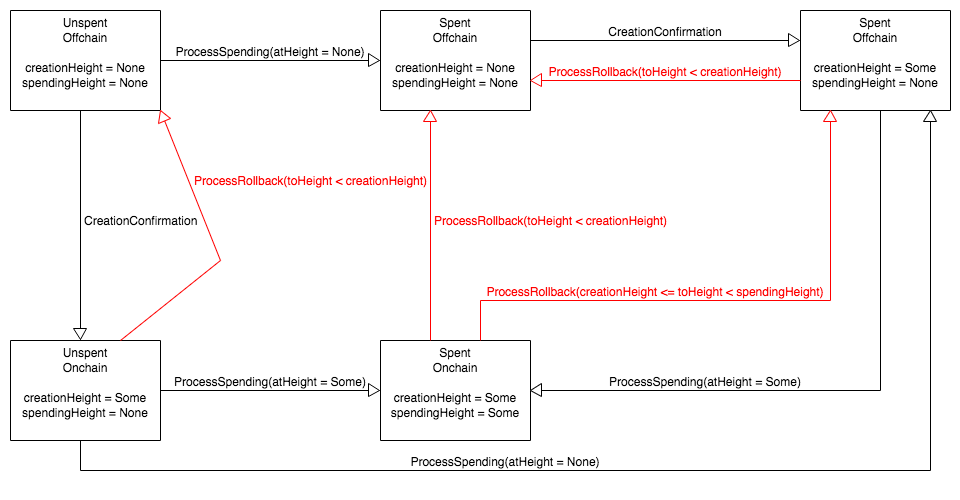
\includegraphics[width=\textwidth]{img/box-transition.png}
    \caption{State transitions for boxes tracked by the wallet
    \label{fig:box-transaction}}
\end{figure}

\end{document}
